\documentclass{beamer}

\usepackage{ccicons}
\usepackage{booktabs}

\newcommand{\shorturl}[2]%
  [?utm\_source=jsc\&utm\_medium=presentation\&utm\_campaign=ox\_open\_sci\_2012]%
  {\href{http://#2#1}{\nolinkurl{#2}}}

\usetheme{Bath}

\title{Technology training for PG students}
\subtitle{Research data management and social media}
\author[Jez Cope]{Jez Cope\\ ICT Project Manager}
\institute[Bath]{Centre for Sustainable Chemical Technologies\\ University of Bath}
\date[22 August 2012]{Oxford Open Science meeting\\ \textit{Wednesday 14 August 2012}}

\AtBeginSection[]
{
  \begin{frame}<beamer>
    \tableofcontents[sectionstyle=show/shaded,subsectionstyle=show/show/shaded]
  \end{frame}
}

%-----------------------------------------------------------------------------
\begin{document}
%%fakesection Front matter
%-----------------------------------------------------------------------------

\begin{frame}[plain]
  \titlepage
\end{frame}

\begin{frame}
  \tableofcontents
\end{frame}

%-----------------------------------------------------------------------------
\section{Introduction}
%-----------------------------------------------------------------------------

\subsection{Who am I?}

\begin{frame}
  \frametitle{Who am I?}
  
  \begin{columns}
    \begin{column}{6cm}
      \begin{itemize}
        \item Computer scientist \& mathematician by training;
        \item Brief flirtation with computational systems biology;
        \item At University of Bath:
          \begin{itemize}
            \item ICT Project Manager, CSCT;
            \item Technical Data Co-ordinator, Research360 project;
          \end{itemize}
      \end{itemize}
    \end{column}
    \begin{column}{4cm}
      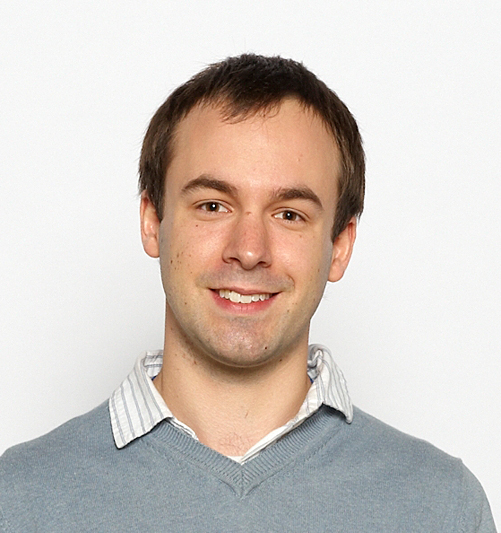
\includegraphics[width=4cm]{COPE_Jez}
    \end{column}
  \end{columns}
\end{frame}

\subsection{Centre for Sustainable Chemical Technologies}

\begin{frame}
  \frametitle{Centre for Sustainable Chemical Technologies}

  \begin{center}
    \includegraphics[width=4cm]{csct-logo-rgb}\\
    \Large\shorturl{bath.ac.uk/csct}
  \end{center}
  
  \begin{itemize}
    \item Cross-disciplinary research centre;
    \item Develop new molecules, materials and processes for sustainability;
    \item EPSRC-funded Doctoral Training Centre.
  \end{itemize}
\end{frame}

\subsection{Research360 project}

\begin{frame}
  \frametitle{Research360 project}
  
  \begin{center}
    \Large\shorturl{blogs.bath.ac.uk/research360}
  \end{center}

  \begin{itemize}
    \item JISC-funded 18 month project;
    \item Develop human \& technical infrastructure for research data management;
    \item Institutional drivers:
      \begin{itemize}
        \item Business continuity;
        \item Openness \& research integrity;
        \item EPSRC expectations;
        \item RCUK common principles.
      \end{itemize}
  \end{itemize}
\end{frame}

%-----------------------------------------------------------------------------
\section{Connected Researcher @ Bath}
%-----------------------------------------------------------------------------

\subsection{What we did}

\begin{frame}
  \frametitle{Social media for researchs}
  
  \begin{itemize}
    \item Attract collaborators;
    \item Attract funding (private/public);
    \item Attract PhD students;
    \item Get more citations;
    \item Debate \& share ideas with peers;
    \item Influence policy;
    \item Knowledge transfer;
    \item Engage with the public.
  \end{itemize}
\end{frame}
\begin{frame}
  \frametitle{Connected Researcher @ Bath}
  
  \begin{itemize}
    \item Aim: To support social media use by researchers;
    \item Entirely grass-roots;
    \item Mixture of events:
      \begin{itemize}
        \item Seminars with invited speakers;
        \item Panel sessions;
        \item Hands-on workshops.
      \end{itemize}
  \end{itemize}
\end{frame}

\subsection{What we found}

\begin{frame}
  \frametitle{Experiences}
  
  \begin{itemize}
    \item Workshops well attended;
      \begin{itemize}
        \item Mostly students, but a few staff too;
      \end{itemize}
    \item Hands-on workshops were popular;
    \item Need to make clear:
      \begin{itemize}
        \item Why social tools are useful;
        \item How to use them to produce \emph{useful results}.
      \end{itemize}
  \end{itemize}
\end{frame}

\begin{frame}
  \frametitle{Going forward}
  
  \begin{itemize}
    \item Well received inside \& outside the university;
    \item Taken up by Researcher Development Unit and Web Services.
  \end{itemize}
\end{frame}

%-----------------------------------------------------------------------------
\section{Research data management}
%-----------------------------------------------------------------------------

\subsection{What we did}

\begin{frame}
  \frametitle{Research Data Management Workshops}
 
  \begin{itemize}
    \item Workshops for PG research students;
    \item Practical, effective strategies for data management;
    \item Treatment of the \emph{whole} research lifecycle.
  \end{itemize}
\end{frame}

\begin{frame}
  \frametitle{Research Data Management Workshops}
  
  \begin{itemize}
    \item Two workshops so far;
    \item DTC students (all chemists/chemical engineers):
      \begin{itemize}
        \item Introduction led by DTC Director (an academic);
        \item Hands-on data management planning;
      \end{itemize}
    \item PGskills (University-wide PGR training)
      \begin{itemize}
        \item Shorter, less hands-on;
      \end{itemize}
  \end{itemize}

  \bigskip
  \shorturl{blogs.bath.ac.uk/research360/category/training/}
\end{frame}

\subsection{What we found}

\begin{frame}
  \frametitle{Attitudes}
  
  \begin{itemize}
    \item Good awareness of the issues\ldots
    \item \ldots but poor level of implementation;
    \item Supportive of the idea of openness\ldots
    \item \ldots but it's a low priority.
  \end{itemize}
\end{frame}

\begin{frame}
  \frametitle{Feedback}
  
  \begin{itemize}
    \item Satisfaction:
      \begin{itemize}
        \item \textbf{95\%} of participants were satisfied with the course;
        \item \textbf{91\%} would recommend the course to others;
        \item \textbf{95\%} found it relevant to their needs.
      \end{itemize}
    \item Intended follow-up:
      \begin{itemize}
        \item "Prepare a management plan"; and
        \item "Back up my data"
      \end{itemize}
  \end{itemize}
\end{frame}

\begin{frame}
  \frametitle{Improvements}
  
  \begin{itemize}
    \item Dropbox \& the cloud;
    \item Engage staff better;
    \item Include data-type-/discipline-specific examples.
  \end{itemize}
\end{frame}

%-----------------------------------------------------------------------------
\section{Conclusions}
%-----------------------------------------------------------------------------

\begin{frame}
  \frametitle{Conclusions}
  
  \begin{itemize}
    \item Postgraduate researchers are:
      \begin{itemize}
        \item Aware of the potential of technology;
        \item Wary of the perceived risks;
        \item Very strategic about how they use their time;
        \item \alert<2->{Open to learning new stuff;}
      \end{itemize}
    \item PGRs are influenced by their supervisors\ldots
    \item \ldots but often influence them right back;
  \end{itemize}
\end{frame}
\begin{frame}
  \frametitle{That's all, folks}

  \begin{center}
    \huge Any questions?

    \pause\small\bigskip\bigskip
    \begin{tabular}{rl}
      \toprule
      Blog        & \shorturl{erambler.co.uk} \\
      Work stuff  & \shorturl{people.bath.ac.uk/jc619} \\
      Twitter     & \shorturl[]{twitter.com/jezcope} \\
      Google+     & \shorturl[]{gplus.to/jezcope} \\
      \bottomrule
    \end{tabular}

    \bigskip
    \small\shorturl[]{github.com/jezcope/oxford-open-science-2012}\\
    \bigskip
    \href{http://creativecommons.org/licenses/by-sa/3.0/}{\ccbysa}
  \end{center}
\end{frame}

\end{document}
